\chapter{Implementation and Testing}
This chapter will highlight the implementation of the mashup and executing it. In general, the working of the mashup works exactly as specified in the scraping program described in Chapter 3. In the next section, we will test the application and assess its working on different search queries.

\section{Implementation}
The complete mashup system comprises of two Python programmes which form the core working components of the mashup. Additionally, the HTML file templates form the structure of the user interface, the results page, a JavaScript and CSS file. All the source code for the project is available in the appendices. In order to execute the mashup, the main.py file has to be compiled. We tested this on a computer with Windows 7.  Windows Powershell or the cmd prompt can be used. Additionally, this was also tested in a Linux environment.

The implementation is relatively straightforward. All the source code files are in a folder called restaurantGO. The program is a local server where the pc’s ip address and its port are initialized in main.py file. Once main.py is executed, the user interface page is opened in the web browser. The mashup is basically designed to accept cuisine name as the user query and it displays the restaurants of that cuisine with predefined categories as specified in the working of the mashup. Hence, the mashup can only display results of restaurant information taken from the restaurant-guide.com which was used for mashing the data.

\section{Testing}

In this section, we execute the mashup using cuisine queries and explain about the details obtained.

Upon executing the mashup with the cuisine query as 'British', one of the obtained results looks as follows(normally, a list of restaurants is obtained and structured).

\begin{figure}[!htb]
  \centering
  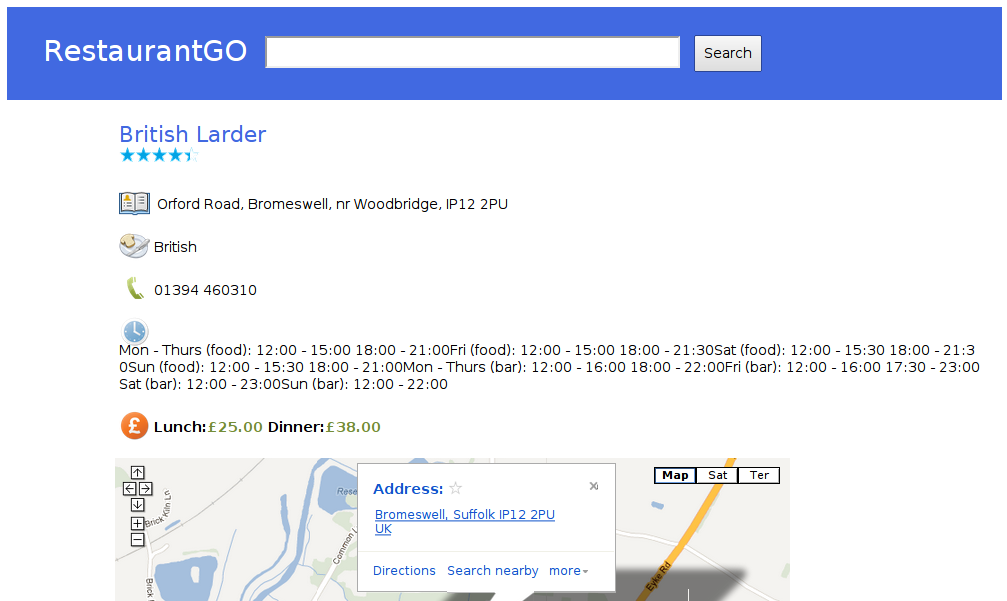
\includegraphics[width=16cm]{fig/restaurant_go_results_british.png}
  \caption[ RestaurantGo search results for  British cuisine]
  {shows search results for British cuisine}
\end{figure}


The above query displays a list of 10 or more restaurants of British cuisine. There also exists an option to choose more results. There are some loading delays which can be attributed to Google maps locations being displayed, which may take a while to load.
The mashups works well with providing a cuisine name as a search query. Similarly, the results for 'Chinese' as the query, are shown in Figure ~\ref{fig:4.2}.

\begin{figure}[!htb]
  \centering
  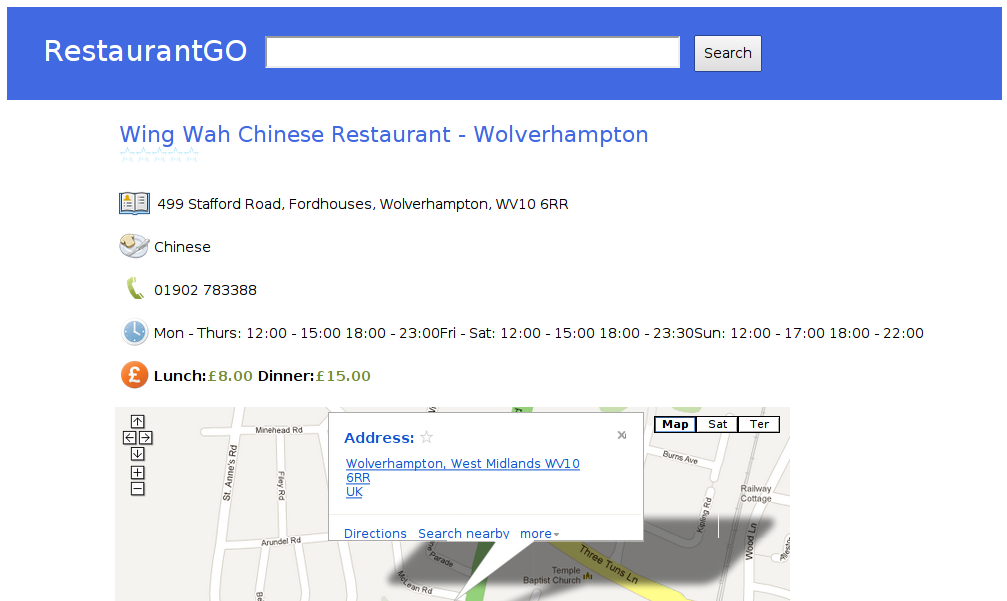
\includegraphics[width=16cm]{fig/restaurant_go_results_chinese.png}
  \caption[ RestaurantGo search results for Chinese cuisine]
  {shows search results for Chinese cuisine}
  \label{fig:4.2}
\end{figure}


With these results, it can be asserted that the mashup works well with cuisine names as queries from the user to get the necessary details of a restaurant's record, such as its address and a Google maps location display for easy navigation. It’s also useful to display the opening and closing times so that the users can plan their schedule and be organized so as to visit the restaurant at their convenience. Budget minded users can check out the prices of the restaurant before making their decision to visit the restaurant.

Moreover, more complex queries, such as 'Italian Coventry' or 'Coventry Italian'(the order does not matter) can also be done, to filter out results for a specific desired location.

Although the mashup works for the cuisines and locations, as in the test case, we did also try it out with some random gibberish text or even normal phrases like “welcome”, “hello” etc. and it produced an error page.
As far as testing of the mashup goes, it works only with cuisine names that are well versed with the restaurant-guide.com website.

\section{Evaluation}
Apart from testing the system, a survey was conducted allowing users to perform an evaluation of the system. Evaluations were recorded based on SUS (System Usability Scale) questionnaire \cite{20} in terms of efficiency, effectiveness and satisfaction. The group of users mainly comes from computer science background. The evaluations are as follows:

\subsection{User 1}
\textbf{Regarding search:}

\begin{itemize}

\item \textbf{Effectiveness} (can users successfully achieve their objectives): I think users can, because the search results cover many types of cuisines, I got numerous results when searched for British, Italian, Indian, Pakistani, African, etc - so all types of keywords get matched. The maps show up each place with postcode, so it helps to straightaway take this info, also quite some important details like opening times, price, phone no, etc. However scope for improvement is that results are mostly in London or Edinburgh, Manchester, Liverpool, etc.. It would help if results are matched based on distance, so I would be more likely to use this system.
\item \textbf{Efficiency} efficiency is pretty fast, and there is hardly any delay, so this is taken care of.
\item \textbf{Satisfaction} (was the experience satisfactory): Apart from the fact that results are ignorant of distance from current location, the search results and the details given are pretty satisfactory. User will be pretty likely of using this system.
  
\end{itemize}

\subsection{User 2}

\begin{itemize}
  
\item \textbf{Effectiveness} The search is quick and efficient. It is able to find all data containing the search tag and displays it in a neat manner.

\item \textbf{Efficiency} It is a quick system and there is little lag between placing a search query and getting results, however since the results are not filtered finding the exact result might be more time consuming.

\item \textbf{Satisfaction} Yes I would say that the experience was satisfactory. 
\item \textbf{Note} I have noticed that your code breaks on unknown search queries, I would recommend you put in some error handing that breaks gracefully and serves up an error message of some sort. Its never nice for a program to break in the back with no indication in the front.

\end{itemize}

\subsection{User 3}

\begin{itemize}
\item \textbf{Effectiveness} (can users successfully achieve their objectives):
        Users are presented with a list of restaurants upon submitting a choice of cuisine. It would be great if the user is given some feedback as to how the results are sorted and/or if the sorting order could be changed on Price or Location (Distance).

\item \textbf{Efficiency} (how much effort and resource is expended in achieving those objectives):
        Results are easily obtained by simply typing in your choice. The results are fetched and presented quickly.

\item \textbf{Satisfaction} (was the experience satisfactory):
        For a single cuisine search, the results were excellent.

\item \textbf{Scope} It might be worthwhile for a future version to offer more than one choices of cuisine to search upon even though the data-source only offers one cuisine type. Additionally, AND and OR logic could be incorporated to support more complex queries.

\end{itemize}

\subsection{User 4}

\begin{itemize}
\item \textbf{Effectiveness} Depends on what the user is searching for , it gives satisfying results when we search with keywords such as cuisine name and  name of the city. But it leaves the user wanting more features such as intelligent searching.

\item \textbf{Efficiency} The application is pretty efficient when it comes to searching with the help of keywords. The results in most of the cases were correct.

\item \textbf{Satisfaction} Much work still needs to go in the application so that it becomes as an application which can be used by a larger amount of people. But on knowing the keywords, the search was pretty efficient and satisfactory.
\end{itemize}

\subsection{User 5}

\begin{itemize}
\item \textbf{Effectiveness} It is clear and easy to use. But I try to enter something like Burmese, it does not seem to like it. Some words seem to work fine, when I run second time.

\item \textbf{Efficiency} It can show the results very quickly actually. Is the result based
on my geographical location?

\item \textbf{Satisfaction} Yes. It would be nice to have something like you are this much away
from this restaurant, or your local alternatives are these.
\end{itemize}

The application was tested by five users and their evaluations were recorded. Overall, users were satisfied with the experience. They did point out some visual formatting issues and lack of an error page for exceptional query searches. For instance,the application doesn't work on non-cuisine names and random text, so this was fixed by providing an output message "search found 0 results". A problem specified by majority of the users that the results are drawn at random and are not based on user's geographical distance. Conducting a test with 5 users was quite advantageous since a common usability problem was detected \cite{27}.